\section{Acquisition of Parameters}\label{sec:Param}

A method to obtain the parameters from the wheel (mass, distance from its center to the pivoting point of the frame, inertia with respect to its center of rotation and friction) is provided in \appref{app:wheelParameters}. However, as these parameters should remain constant and they have been obtained by previous project runners, it is chosen to use these known parameters\cite{SVJohansen}.

\begin{table}[H]
	\begin{tabular}{|l|l|p{3cm}|}
		\hline %-----------------------------------------------------------------------------------
		\textbf{Parameter} &\textbf{Value} &\textbf{Units}\\
		\hline %-----------------------------------------------------------------------------------
		\si{m_w}         & \si{0,222}       &kg\\
		\hline
		%-----------------------------------------------------------------------------------
		\si{l_w}         & \si{0,093}       &m\\
		\hline %-----------------------------------------------------------------------------------
		\si{J_w}         & \si{0,601 \cdot 10^{-3}}	&\si{kg \cdot m^2}\\
		\hline  
		%-----------------------------------------------------------------------------------
		\si{B_w}         & \si{17,03 \cdot 10^{-6}}       &N \si{\cdot m \cdot s \cdot rad^{-1}}\\
		\hline
	\end{tabular}
	\caption{Parameters of the wheel}
	\label{ParametersWheel}
\end{table}

On the other hand, the rest of the parameters (\si{m_F, l_F, J_F\ and\ B_F}) which are related to the frame must be found out. This is due to the addition of the electronics to the frame, which were not there when the tests were made in previous projects.

\subsection{Mass of the Frame}
The first one to find is the mass of the frame, which can be measured by weighing the setup without the base and substracting the known mass of the wheel. This gives a mass of \si{0,548\ kg}.

\subsection{Center of Mass of the Frame}
The new center of mass can be found hanging the frame from different corners and measuring the deviation angle from the vertical position in every direction. This gives a center of mass which can be seen in \figref{centerOfMassDiagram}. 
\begin{figure}[H]
	\centering
	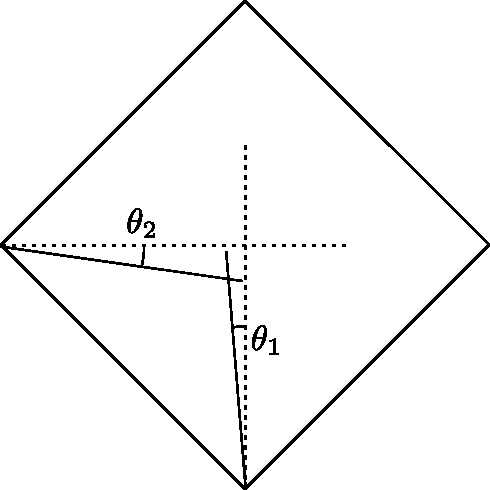
\includegraphics[scale=0.6]{figures/centerOfMassDiagram}
	\caption{Location of the center of mass, where \si{\theta_1=0,043\ rad\ and\ \theta_2=0,078\ rad}}
	\label{centerOfMassDiagram}
\end{figure}


The new point is not in the vertical line as it was assumed in the model, but this can be solved correcting the offset in the calculation of the angle inside the control loop and taking this new point as the equilibrium one. 

The new \si{l_F} can then be obtained projecting the center of mass onto the vertical line, resulting in \si{8,498\ cm}.

\subsection{Inertia and Friction of the Frame}
In the previous sections parameters have been found, however, some critical parameters were given from a previous project. When these parameters were found, the Cubli had another mass, due to some physical modifications of the platform, which were performed after the refereed project. The critical parameters are \si{J_F} and \si{B_F}. If the model is compared with reality, as seen on \figref{InitialModelParameterCompare}, it is evident that some further tuning of the parameters is needed.

\begin{figure}[H] 
	\centering
	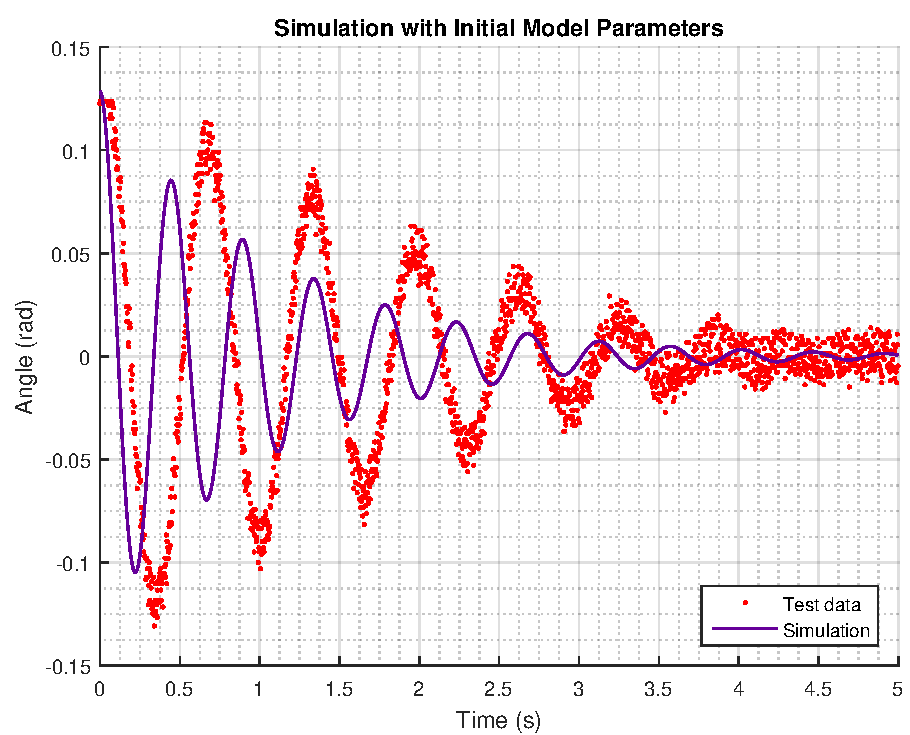
\includegraphics[width=.6\textwidth]{figures/InitialModelParameterCompare}
	\caption{A comparison of the model simulation and the initially given parameters (\si{J_F=6,08 \cdot 10^{-3}\ kg \cdot m^2\ and\ B_F=5,32 \cdot 10^{-3}\ m \cdot s \cdot rad^{-1}})}
	\label{InitialModelParameterCompare}
\end{figure}
%
This problem can be solved using optimization, which is the subject of the proceeding section.\fxnote{Include Senstools manual and reference it here}